\subsubsection{\stid{4.01} \dataviz\ Software Development Kits} 

\paragraph{\textbf{DataViz SDK Overview}}
\paragraph{}

The Data \& Visualization (DataViz) SDK aims to create a production-quality infrastructure necessary to manage, share, and facilitate data analysis of mission-critical codes at scale. The project focuses on community development and a commitment to success via quality improvement policies, better build and deployment processes, and the ability to use diverse, independently developed DataViz SDK projects, in combination, for data analysis and visualization problems.

The DataViz SDK's responsibility is to coordinate the development, testing, and deployment activities for the suite of projects across the ECP Data \& Visualization area as it applies to cross-project interoperability, and develop the necessary tooling and shared infrastructure to serve these goals. This coordination's resulting product is a unified set of usable, standardized, and interoperable packages ready for the upcoming exascale machines. We have designed the efforts to support the DataViz SDK to fit within the overarching goal of leveraging and integrating data management, analysis, and visualization techniques developed across the ECP ST ecosystem to support scientific discovery and understanding.

In addition, DataViz SDK provides a capability supporting collaborative analysis and visualization software development, helping independent teams accelerate the adoption of best practices, enabling interoperability of independently developed software, and improving developer productivity and sustainability of the software products.

\paragraph{\textbf{Key Challenges}}
\paragraph{}

Scientists and engineers from various research cultures and significantly different software engineering maturity levels develop Data \& Visualization software packages. In addition to the challenges outlined in Section~\ref{subsubsect:ecosystem-sdk}, ECP Data \& Visualization software packages will use different combinations of dependency software in various configurations. Visualization applications and libraries, in particular, utilize lower-level graphics libraries from an OpenGL stack needing to be reliably mapped to a diverse set of underlying hardware.  These applications demand the deployment infrastructure supporting the appropriate combination of software and hardware-based rendering on NVIDIA, AMD, or Intel GPUs and accelerated offscreen rendering APIs like EGL.  Requirements such as these place the DataViz SDK between the hardware teams and the analysis and visualization software developers preparing to run on new architectures yet delivered by ECP.

DataViz SDK software packages also have, on average, a much deeper dependency tree than is typical within HPC.  As of this writing, the optimized set of thirteen ECP DataViz SDK packages requires over 201 dependencies.  Many packages share these dependencies, each with their own set of constraints.  This combination presents a unique challenge to ensure compatibility, interoperability, and reliability of the entire stack as a whole, beyond the individual packages.

\paragraph{\textbf{Solution Strategy}}
\paragraph{}

First, the DataViz SDK solution strategy involves pursuing usability, standardization, interoperability, and sustainability goals through a set of community policies to improve software practices. The DataViz SDK community policy tasks have required us to define a common terminology for effective communication.

Second, we leverage shared infrastructure, such as the Spack~\cite{gamblin+:sc15} package manager and CI testing at ECP facilities. We have built the SDK release and delivery deployment goals on Spack as a unifying package manager, while our reliability and sustainability goals benefit from and leverage a combination of CI testing infrastructure from upstream Spack, DOE facilities, and dedicated project resources.

Finally, we define a spack meta-package, ecp-data-vis-sdk, to enable the delivery of ECP targeted configurations of data and visualization packages through E4S.  The meta-package establish dependencies for the packages within the DataViz SDK, and serves as the backbone of our interoperability testing and deployment efforts. It enables the coincident optimized deployment of the diverse set of packages in the ECP Data \& Visualization portfolio:
\begin{itemize}
\item Visualization tools and libraries
  \begin{itemize}
  \item ASCENT, Catalyst, Cinema, ParaView, and VTK-m
  \end{itemize}
\item Data reduction and compression libraries
  \begin{itemize}
  \item SZ and ZFP
  \end{itemize}
\item I/O and data service libraries
  \begin{itemize}
  \item ADIOS, Darshan, HDF5, PNetCDF, UnifyFS, VeloC
  \end{itemize}
\end{itemize}

\noindent
The packages contained in the meta-package are able to be deployed in a way that enables all of the appropriate features for each package when the others are present and in a way that satisfies one anothers dependencies. The release strategy in the early efforts of the SDK was to push product readiness for inclusion in the E4S releases by assisting individual packages with Spack packaging and CI testing. With that effectively achieved in the early efforts of the SDK our focus has now shifted to the collective interoperable deployment and testing of all the packages on targeted ECP platforms of interest.

\paragraph{\textbf{Recent Progress}}
\paragraph{}

% \textit{SENSEI}

\textit{Integration with upstream Spack CI} The spack package manager is the distribution mechanism of choice for ECP.  To ensure reliability for it's packages the spack project has developed a CI capability for specific package collections of interest to be built and validated in every pull request.  Through coordination with the spack project, the DataVis SDK has integrated it's spack meta-package as one of the primary pipelines of interest for the spack project. As a result, the packages and dependencies enabled by the DataVis SDK are validated for build correctness on every change and addition to spack.

\textit{Deployment on Spock} The Frontier system at OLCF is scheduled to come online by the end of 2021 or early 2022. In preparation we have targeted Spock, the testing and development environment for Frontier, for an initial full deployment of the DataVis SDK.  We have now successfully been able to deploy the ecp-data-vis-sdk meta-package on the Spock system using the Cray Programming Environment with both GNU and Cray compilers while enabling twelve distinct Data \& Vis packages.  This will minimize the effort needed to deploy on Frontier when it comes online.

\paragraph{\textbf{Next Steps}}
\paragraph{}

We highlight our next steps in the follow on project milestones.

\textit{STDV01-38} --- Implement and test accelerator variants in the SDK: The initial SDK package lacks the necessary features to enable and propagate GPU features for the packages.  We will implement and test GPU options in the SDK for each of the accelerator platforms of interest (AMD, NVIDIA, and Intel) and ensure they are consistently and reliably applied to the DataVis SDK pacakges.

\textit{STDV01-39} --- Deployment of the SDK into E4S: We will integrate the ecpdata-vis-sdk spack meta-package into the E4S distribution and it will become the provider-of-choice for the ECP Data \& Visualization packages it supports.  This will ensure that E4s will provide the most effective and useful configurations of these packages.

\textit{STDV01-40} --- Deployment of the SDK in facility environments: We will deploy the full SDK on the various ECP platforms available in production.  This will ensure that when Data \& Vis packages are provided via spack by facilities then they are in the most effective and useful configuration possible for their users.

\paragraph{HDF5}
\paragraph{Overview}
\paragraph{}
HDF5 is a data model, I/O library, and file format to store and manage data. It supports an unlimited variety of datatypes, and is designed for flexible and efficient I/O for high volume and complex data. Its extensive ecosystem is illustrated by over 2,000 repositories on GitHub depending on HDF5 or 160 packages in Spack along with many third-party tools that support HDF5, e.g., MATLAB, and open source packages, e.g., h5py, Pandas, Keras, and TensorFlow. 

HDF5 is portable and is extensible, allowing applications to evolve in their use of HDF5. It supports many different types of data stores, such as local, clustered, and networked file systems and object stores. HDF5 is highly customizable through its purposefully designed extension interfaces, Virtual Object Layer (VOL) and Virtual File Driver (VFD) interfaces as shown in Figure~\ref{fig:HDF5-Arch}.
\begin{figure}[htb]
    \centering
    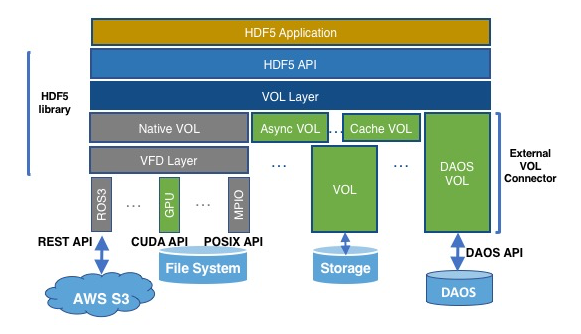
\includegraphics[width=0.75\textwidth]{projects/2.3.4-DataViz/2.3.4.01-DataViz-SDK/HDF5-Arch-small.png}
    \caption{\label{fig:HDF5-Arch}
    HDF5 architecture: green rectangles represent dynamically loaded VFD and VOL connectors to access data on different storage devices; grey and blue rectangles represent components of the HDF5 library.}
\end{figure}

 The most recent extensions include support for Intel DAOS high-performance storage and NVidia’s GPUDirect interface for data movement between storage and GPU memory. 
Numerous ECP applications use HDF5 or high-level libraries built on top of HDF5 (for example, H5Part) for data management. Therefore, HDF5 is a critical part of the Data \& Vis SDK. 

The HDF Group team’s responsibility is to maintain HDF5 on the ECP systems, develop enhancements to boost the performance of the ECP HDF5 applications; integrate enhancements developed by other ECP teams (e.g. DataLib, ExaIO); and deliver HDF5  to the ECP users as a part of the Spack package and Data \& Vis SDK. 

\paragraph{Key  Challenges}
\paragraph{}

The HDF Group team faces two major challenges. The first challenge is extending HDF5 legacy software to deliver high-performing features for the Exascale systems while maintaining HDF5 current performance standards and avoiding HDF5 software disruption for the millions of non-HPC users. The second challenge is the complexity of the HDF5 software that may lead to its misapplication, resulting in poor performance, especially in the HPC environment. The third challenge is delivering contributions to HDF5 created by other teams promptly and according to HDF5 regression testing and coding standards.

\paragraph{Solution Strategy}
\paragraph{}
To lower the barrier for adopting HDF5 by ECP applications and delivering new features timely, The HDF Group (1) provides HDF5 software that is regularly tested on and released for ECP platforms, (2) integrates newly developed features into mainstream HDF5 and makes them promptly available via Spack and Data \& Vis SDK, (3) educates HDF5 users on the best HDF5 practices and new features, and (4) works closely with ECP teams on features development and applications’ tuning. 

\paragraph{Recent Progress}
\paragraph{}
In 2021, The HDF Group developers made enhancements to the HDF5 library to address requirements of the HDF5 ExaIO VOL connectors - \href{https://github.com/hpc-io/vol-async}{Async}, \href{https://github.com/hpc-io/vol-external-passthrough}{Pass-through} and \href{https://github.com/hpc-io/vol-cache}{Cache} VOL connectors, and \href{https://github.com/hpc-io/vfd-gds}{NVIDIA GPU Direct I/O VFD}. The requested changes are available in the \href{https://github.com/HDFGroup/hdf5}{HDF5 develop branch} on GitHub and will be released in the HDF5 1.13 series of releases and later. The releases can be obtained from The HDF Group \href{https://portal.hdfgroup.org/display/support/Downloads}{website} or using the Spack package manager.  

We performed a major refactoring of internal HDF5 library APIs to accommodate new \href{https://portal.hdfgroup.org/display/HDF5/Asynchronous+operations+with+HDF5+VOL+connectors}{asynchronous APIs}.  New HDF5 APIs are designed for HDF5 VOL connectors that support asynchronous operations using the \href{https://portal.hdfgroup.org/display/HDF5/Event+Set}{HDF5 Event Set APIs}. This feature allows I/O to proceed in the background while the application performs other tasks. 

HDF5 VOL and VFD APIs were reworked to address the issues brought up by the ExaIO developers. We held a webinar on the changes to help HDF5 VOLs and VFDs developers with porting existing connectors to the new version of the HDF5 library. Recording and slides are available from \href{https://www.hdfgroup.org/2021/09/webinar-followup-new-features-in-the-hdf5-1-13-0-release/}{The HDF Group website}. 
ECP ExaIO VOL connectors were integrated with Spack. The HDF Group also worked with the ExaIO team on coordination of the HDF5 library and VOL connectors releases.

CI testing was set up to keep HDF5 VOL connectors development and the HDF5 library development in sync. During our integration and testing work, we addressed several issues and desired improvements reported by the DataLib and ExaIO teams. We added a feature that allows auto-detection of a VOL connector used to open an HDF5 file; the feature is available in HDF5 1.13.0 and HDF5 1.12.2 and later maintenance releases; we made improvements to collective metadata write operations and addressed the issues found when using IBM SpectrumScale MPI on the Summit system.

The required changes to the HDF5 library architecture for supporting HDF5 VOL connectors added 7-10\% overhead for the applications that do not use connectors at all. The overhead was especially prominent for applications that work with a lot of HDF5 objects. We identified and implemented several optimizations and saw up to 10\% reduction in time spent by a \href{https://jira.hdfgroup.org/browse/HDFFV-9671}{benchmark} provided to us by LLNL. 

Other integration work includes support for SZ and ZFP compression filters in the maintenance releases of the HDF5 library starting with the HDF5 1.10.7 release. The HDF Group developers also investigated HDF5 performance with SZ and ZFP HDF5 compression filters. Our study showed that HDF5 filters pipeline implementation doesn't create additional overhead for SZ and ZFP compressions.

In 2021, The HDF Group continued with \href{https://www.hdfgroup.org/category/hdf5-resources-for-ecp-users/}{outreach activities}. Recent activities included two Tutorials \href{https://www.hdfgroup.org/2021/05/webinar-followup-hdf5-application-tuning-there-is-more-than-one-way-to-skin-a-catfish-part-2/} {"HDF5 Application Tuning"} and \href{https://www.hdfgroup.org/2021/09/webinar-followup-new-features-in-the-hdf5-1-13-0-release}{"New features in HDF5 1.13.0"}, and a \href{https://portal.hdfgroup.org/pages/viewpage.action?pageId=73924784}{white paper}. The HDF team delivered HDF5 tutorial for ECP 2021 annual meeting and gave a talk on the new ECP VOL/VFD features at the HDF5 BoF at the annual meeting.

\paragraph{Preliminary Experiences on Early Access systems}
\paragraph{}
The HDF5 software has been tested regularly with and without Spack on Arcticus, Theta, ThetaGPU, Spock, Crusher and Perlmutter.  In the absence of GitLab testing framework, we have set up our own custom automated regression testing on Theta and Crusher with results posted to \href{https://cdash.hdfgroup.org}{CDash}.  We will extend this approach to other EAS until GitLab is available.  We didn't encounter any particular problems with porting and testing our software.  Along with HDF5 software, we also ported and tested \href{https://portal.hdfgroup.org/display/support/Registered+VOL+Connectors}{HDF5 VOL connectors} created by ECP teams on targeted EAS.  The \href{https://portal.hdfgroup.org/pages/viewpage.action?pageId=74188097}{Cuda GPU VFD} was tested on ThetaGPU and is available in the hdf5-vfd-gds Spack package.  It was dicovered in testing that running tests with hdf5-vfd-gds on ThetaGPU required setting the Spack stage directory to the Lustre filesystem in order for the test to pass.  Applications using CUDA GPU VFD should be run only on a parallel filesystem. 

\paragraph{Next Steps}
\paragraph{}
The HDF Group activities will continue in two areas:  productization of the HDF5 features developed for ECP applications and outreach. In 2022, we will continue with CI testing on ECP systems and will provide maintenance releases of the HDF5 library.  We will deliver a TOOLKIT for the VOL connectors developers to facilitate the development of new HDF5 connectors. We will integrate HDF5 subfiling VFD and multi-dataset feature (access data in multiple datasets using a single I/O call) that we are developing under the ExaIO project and release it in the mainstream HDF5. We will continue working with the ECP HDF5 applications teams on I/O performance, conduct Tutorials and Webinars, and create additional documentation on efficient usage of HDF5 in the ECP HPC environment. 
